\documentclass[a4paper,oneside]{article}

\usepackage[T1]{fontenc}
\usepackage[utf8]{inputenc}
\usepackage[english]{babel}

\usepackage[margin=2.54cm]{geometry}
\usepackage{amsmath}
\usepackage{siunitx}
\usepackage{listings}
\usepackage{color}
\usepackage{textcomp}
\usepackage{graphicx}
\usepackage{subcaption}
\usepackage[section]{placeins}
\usepackage{hyperref}

\definecolor{matlabgreen}{RGB}{28,172,0}
\definecolor{matlablilas}{RGB}{170,55,241}

\newcommand{\includecode}[1]{\lstinputlisting[caption={\ttfamily #1.m},label={lst:#1}]{matlab/#1.m}}
\newcommand{\textinlinecode}[1]{\lstinline[basicstyle=\ttfamily,keywordstyle={},stringstyle={},commentstyle={\itshape}]{#1}}
\newcommand{\inlinecode}[1]{\ifmmode\text{\textinlinecode{#1}}\else\textinlinecode{#1}\fi}

\renewcommand{\vec}[1]{\overline{#1}}
\renewcommand{\Re}[1]{\operatorname{Re}\left[#1\right]}
\newcommand{\E}[1]{\operatorname{E}\left[#1\right]}
\newcommand{\norm}[1]{\left\lVert#1\right\rVert}
\newcommand{\abs}[1]{\left|#1\right|}
\newcommand{\F}[1]{\operatorname{\mathcal{F}}\left[#1\right]}
\newcommand{\ceil}[1]{\left\lceil#1\right\rceil}
\newcommand{\floor}[1]{\left\lfloor#1\right\rfloor}
\newcommand{\Prob}[1]{\operatorname{P}\left[#1\right]}
\newcommand{\ProbC}[2]{\operatorname{P}\left[#1\middle|#2\right]}
\newcommand{\ind}[1]{\operatorname{\mathbbm{1}}\left\{#1\right\}}
\newcommand{\distr}[0]{\sim}
\newcommand{\unif}[1]{\mathcal{U}_{#1}}

\author{Riccardo Zanol}
\title{Laboratory 6}

\begin{document}
\lstset{
  language=Matlab,
  basicstyle={\ttfamily \footnotesize},
  breaklines=true,
  morekeywords={true,false,warning,xlim,ylim},
  keywordstyle=\color{blue},
  stringstyle=\color{matlablilas},
  commentstyle={\color{matlabgreen} \itshape},
  numberstyle={\ttfamily \tiny},
  frame=leftline,
  showstringspaces=false,
  numbers=left,
  upquote=true,
}
\maketitle

To estimate the motion from one frame to the next some features are
first extracted using the Harris corner detector (limiting the number
of returned features to \inlinecode{corner_max_num}), because it would
be very time consuming to run the Lucas-Kanade algorithm on every
pixel in each frame. Then the gradients $I_x$, $I_y$ and $I_t$ are
computed over the whole frame, the spatial ones are computed using the
built-in Matlab function \inlinecode{imgradientxy}, which uses the
Sobel mask by default, while the temporal gradient is approximated
with
\begin{equation}
  I_t(x,y,t) = \frac{I(x,y,t+1) - I(x,y,t-1)}{2} .
\end{equation}
In this and the following steps the color information is ignored and
the image is converted to gray-scale.

For each feature point $(x_j, y_j)$ a window of $2W+1$ by $2W+1$
pixels is taken from the gradients, centered in $(x_j, y_j)$, so the
optical flow equations for the pixels of the window can be written as
\begin{align}
  \begin{bmatrix}
    I_x(\vec{p_1}) & I_y(\vec{p_1}) \\
    I_x(\vec{p_2}) & I_y(\vec{p_2}) \\
    \vdots & \vdots \\
    I_x(\vec{p_{N_W}}) & I_y(\vec{p_{N_W}}) \\
  \end{bmatrix}
  \begin{bmatrix}
    u \\ v
  \end{bmatrix}
  &= - \begin{bmatrix}
    I_t(\vec{p_1}) \\
    I_t(\vec{p_2}) \\
    \vdots \\
    I_t(\vec{p_{N_W}}) \\
  \end{bmatrix} \\
  A \begin{bmatrix} u \\ v \end{bmatrix} &= - b
\end{align}
where $(u,v)$ is the velocity of the motion that should be estimated
and $\vec{p_i} \in \{ (-W + x_j,\dots W + x_j) \times (-W + y_j,\dots
W + y_j)\}$.  Finally, the motion $(u,v)$ of the window around each
feature point is obtained from the least squares solution:
\begin{align}
  A^TA \begin{bmatrix} u \\ v \end{bmatrix} &= -A^Tb \\
  \begin{bmatrix} u \\ v \end{bmatrix} &= -\left(A^TA\right)^{-1}A^Tb .
\end{align}
The window used in every video has the suggested value for $W=7$.

Since the accuracy of the estimate depends on the eigenvalues of
$A^TA$, which is also the second moment matrix used in the Harris
corner detector, the features are classified according to the
magnitude of the eigenvalues and their ratio in three cases:
\begin{itemize}
  \item when $\lambda_1, \lambda_2 \geq
    \inlinecode{corner_eig_thresh}$ and
    $\frac{\lambda_{max}}{\lambda_{min}} <
    \inlinecode{corner_eigratio_thresh}$ the intensity varies a lot in
    every direction so the feature point is a corner,
    \item when $\lambda_1, \lambda_2 \geq
      \inlinecode{corner_eig_thresh}$ but $\lambda_{max} \geq
      \lambda_{min} \cdot \inlinecode{corner_eigratio_thresh}$ the
      intensity varies a lot only in one direction so the feature
      point is an edge,
    \item in the other cases the eigenvalues are small so the feature
      point is inside a uniform region.
\end{itemize}
In the output videos, these points and a scaled version of their
motion are drawn in, respectively, green, blue and red. In every
tested video the suggested parameters $ \inlinecode{corner_eig_thresh}
= 10000$ and $ \inlinecode{corner_eigratio_thresh} = 10$ seem to
produce good results.

In the simple examples where one or two toy cars move horizontally
across the frame (\inlinecode{car1.avi} and \inlinecode{car2.avi})
this algorithm is able to track the motion using less than 50 feature
points extracted from the Harris detector. Even when the two cars are
very close most of the motion vectors point in the same direction,
except for some points which move as if they were part of the car
moving in the opposite direction. An example of the detected motion
vectors is shown is Fig.~\ref{fig:car1}~and~\ref{fig:car2}.
\begin{figure}[htbp]
  \centering
  \begin{subfigure}{0.5\textwidth}
    \centering
    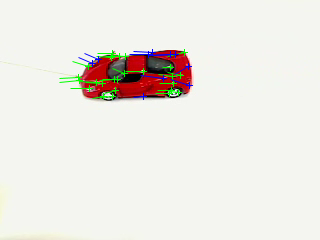
\includegraphics[width=0.95\textwidth]{car1_example}
    \caption{\inlinecode{car1.avi}}
    \label{fig:car1}
  \end{subfigure}%
  \begin{subfigure}{0.5\textwidth}
        \centering
    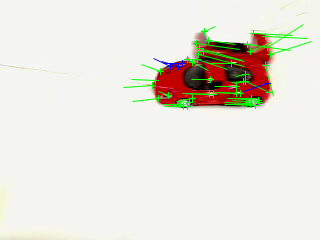
\includegraphics[width=0.95\textwidth]{car2_example}
    \caption{\inlinecode{car2.avi}}
    \label{fig:car2}
  \end{subfigure}
  \caption{Examples from the two videos with the toy cars. The motion
    vectors are scaled by 100}
\end{figure}

In a more complex example, where the camera is moving instead of the
toy car, it can be seen that it is difficult for this algorithm to
correctly estimate fast motion. As an example, in
Fig.~\ref{fig:fast_motion} the camera is moving upward, but a lot of
the estimated motion vectors do not point downward. In another example
(Fig.~\ref{fig:slow_motion}) the camera is moving more slowly toward
the car and it can be seen that the motion vectors are mostly
correct. Also in this video the maximum number of extracted features
was 50.
\begin{figure}[htbp]
  \centering
  \begin{subfigure}{0.5\textwidth}
    \centering
    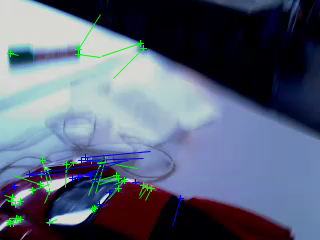
\includegraphics[width=0.95\textwidth]{fast_moving_cam}
    \caption{Fast motion}
    \label{fig:fast_motion}
  \end{subfigure}%
  \begin{subfigure}{0.5\textwidth}
        \centering
    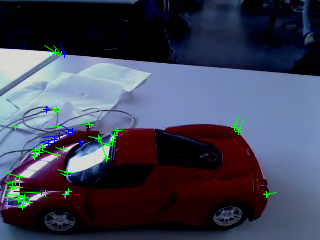
\includegraphics[width=0.95\textwidth]{slow_moving_cam}
    \caption{Slow motion}
    \label{fig:slow_motion}
  \end{subfigure}
  \caption{Examples from \inlinecode{test_ferrari_moving_cam.mp4}. The
    motion vectors are scaled by 100}
\end{figure}

When the camera rotates the algorithm estimates better the motion of
the points in the background that those of the car and during all the
video the corner of the table is one of the better tracked points,
since there is a very sharp change in intensity.

In a video with more moving elements, like \inlinecode{test_room.mp4},
the limit on the number of features must be increased to track all the
moving elements: with just 50 features like in the previous examples
the hand-waving in the background is completely missed, while using
200 features the algorithm is able to follow it. Even the movement of
the person on the chair in the foreground is not followed so well
with just 50 points because of the low contrast with the floor
(Fig.~\ref{fig:chair}).
\begin{figure}[htbp]
  \centering
    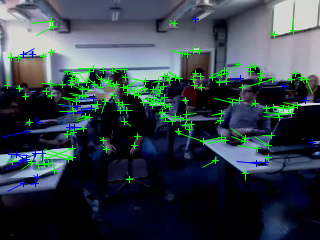
\includegraphics[width=0.6\textwidth]{chair}
    \caption{Example from \inlinecode{test_room.mp4} with 200 feature
      points and the motion vectors scaled by 100}
    \label{fig:chair}
  \end{figure}
\end{document}
